% ============================================================
% CHAPITRE 7
% ============================================================
\chapter{Le tableau de bord d'investigation}
\label{ch:dashboard}

\section{Cinq onglets, un parcours d'analyste}
Le tableau de bord (\fichier{graph\_network\_dashboard.py}, Streamlit) suit le
parcours d'un analyste : voir ce qui se passe, choisir une alerte,
l'investiguer, élargir au réseau, puis vérifier que la plateforme est saine
et que l'historique est fiable (tableau~\ref{tab:onglets}). Il lit le
lakehouse avec \fichier{delta-rs}, une implémentation de Delta Lake sans JVM :
il démarre en quelques secondes et ne consomme aucune ressource Spark.

\begin{table}[htp]
\centering\small
\begin{tabular}{@{}l>{\raggedright\arraybackslash}p{6.0cm}>{\raggedright\arraybackslash}p{5.2cm}@{}}
\toprule
\sffamily\bfseries Onglet & \sffamily\bfseries Contenu & \sffamily\bfseries Source\\
\midrule
\ico{F05B}~Vue d'ensemble & indicateurs clés, réseau suspect en direct, dernières alertes expliquées & gold, silver \fichier{traffic\_windows}\\
\ico{F0F3}~Alertes \& investigation & table filtrable, sous-graphe PyVis de l'alerte, score détaillé, fiche PDF & gold (alertes, sommets, arêtes)\\
\ico{F542}~Explorateur de réseau & voisinage à 1 ou 2 sauts d'un compte, flux entrant et sortant, PageRank & bronze, silver \fichier{account\_metrics}\\
\ico{F013}~Santé du pipeline & durée des micro-batchs par étape, latence, débit, rejets & journaux \fichier{metrics/*.jsonl}\\
\ico{F1C0}~Audit Delta Lake & partitions, historique des versions, \emph{time travel} & journal \fichier{\_delta\_log}\\
\bottomrule
\end{tabular}
\caption{Les cinq onglets du tableau de bord.}
\label{tab:onglets}
\end{table}

Deux conventions visuelles valent pour tous les graphes : la \textbf{couleur}
d'un compte ou d'une alerte est celle de son niveau de risque, toujours
accompagnée de son libellé ; la \textbf{forme} d'un sommet indique son rôle
dans le schéma (étoile : origine, losange : pivot, triangle : mule, carré :
destination). La barre latérale permet d'\textbf{injecter une fraude} de
n'importe quel type en direct, ce qui rend la démonstration reproductible
devant un jury.

\begin{figure}[htp]
\centering
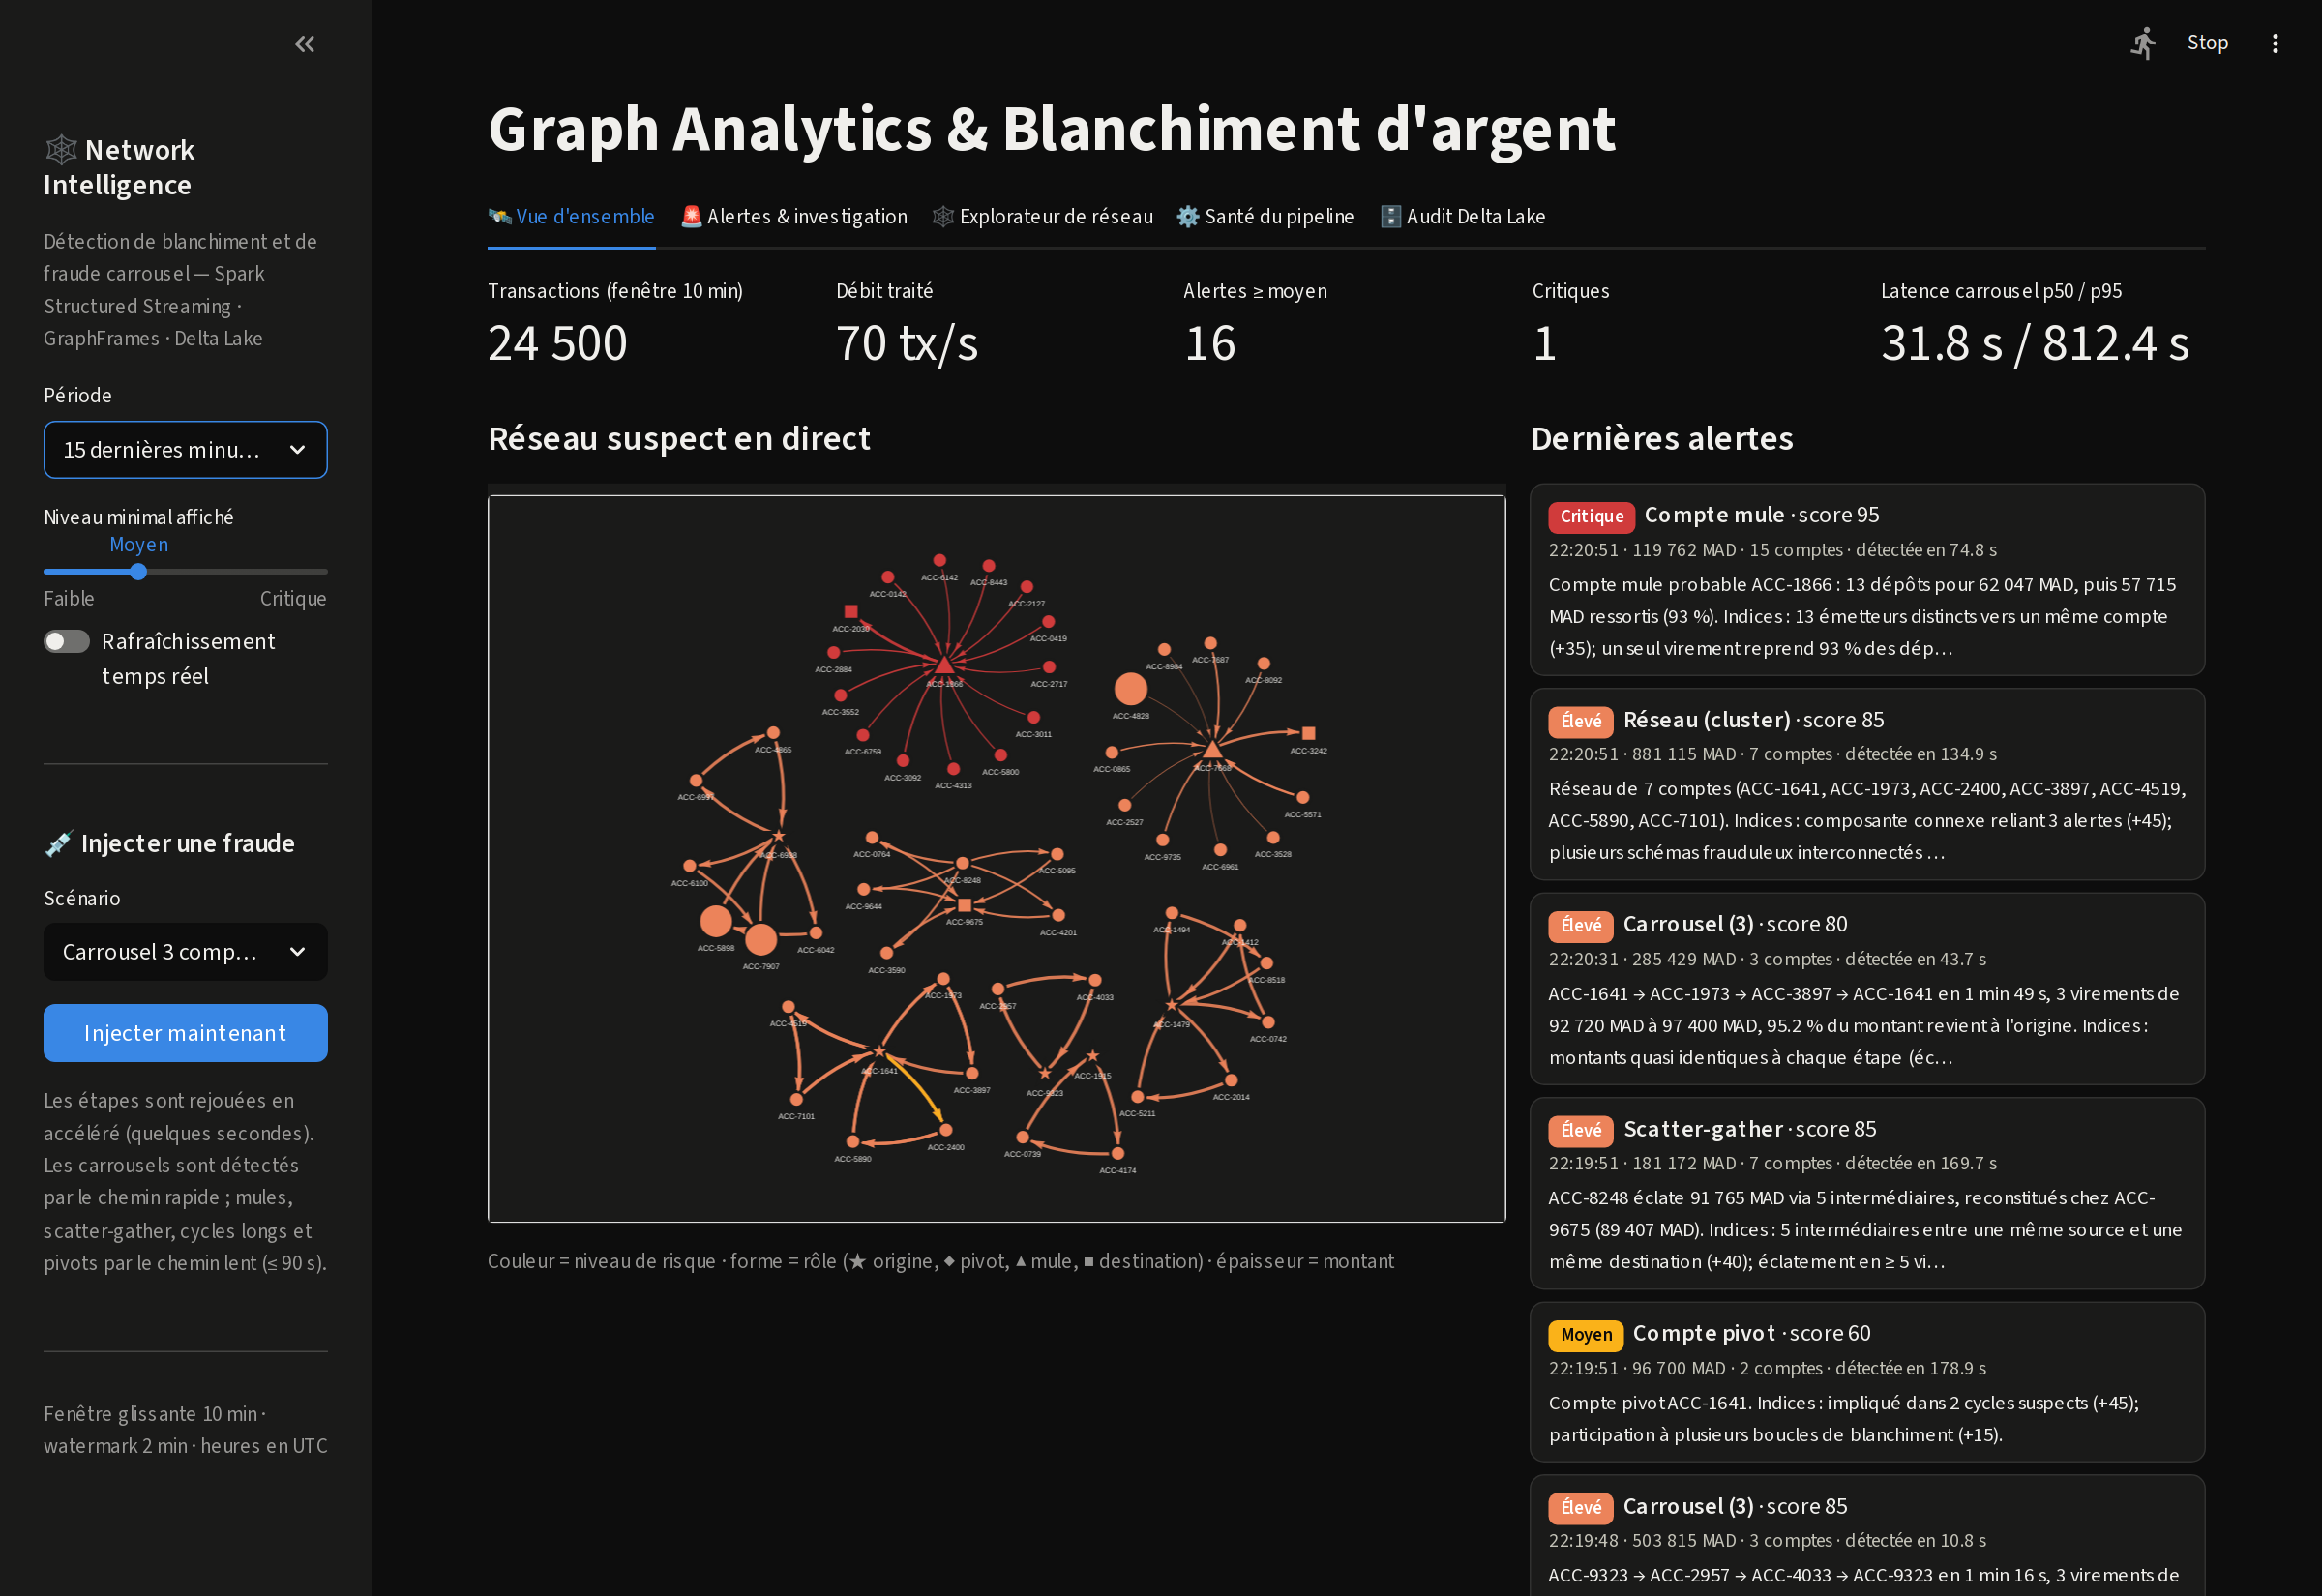
\includegraphics[width=\linewidth]{figures/captures/dashboard_vue_ensemble.png}
\caption[Vue d'ensemble du tableau de bord]{Vue d'ensemble pendant un fonctionnement réel : indicateurs
de la fenêtre courante, réseau suspect (tous les sous-graphes des alertes récentes) et dernières
alertes avec leur explication. Capture prise 7~minutes après un redémarrage : les latences affichées
incluent le rattrapage des messages accumulés pendant l'arrêt (valeurs en régime établi au
chapitre~\ref{ch:resultats}).}
\label{fig:dash1}
\end{figure}

\begin{figure}[htp]
\centering
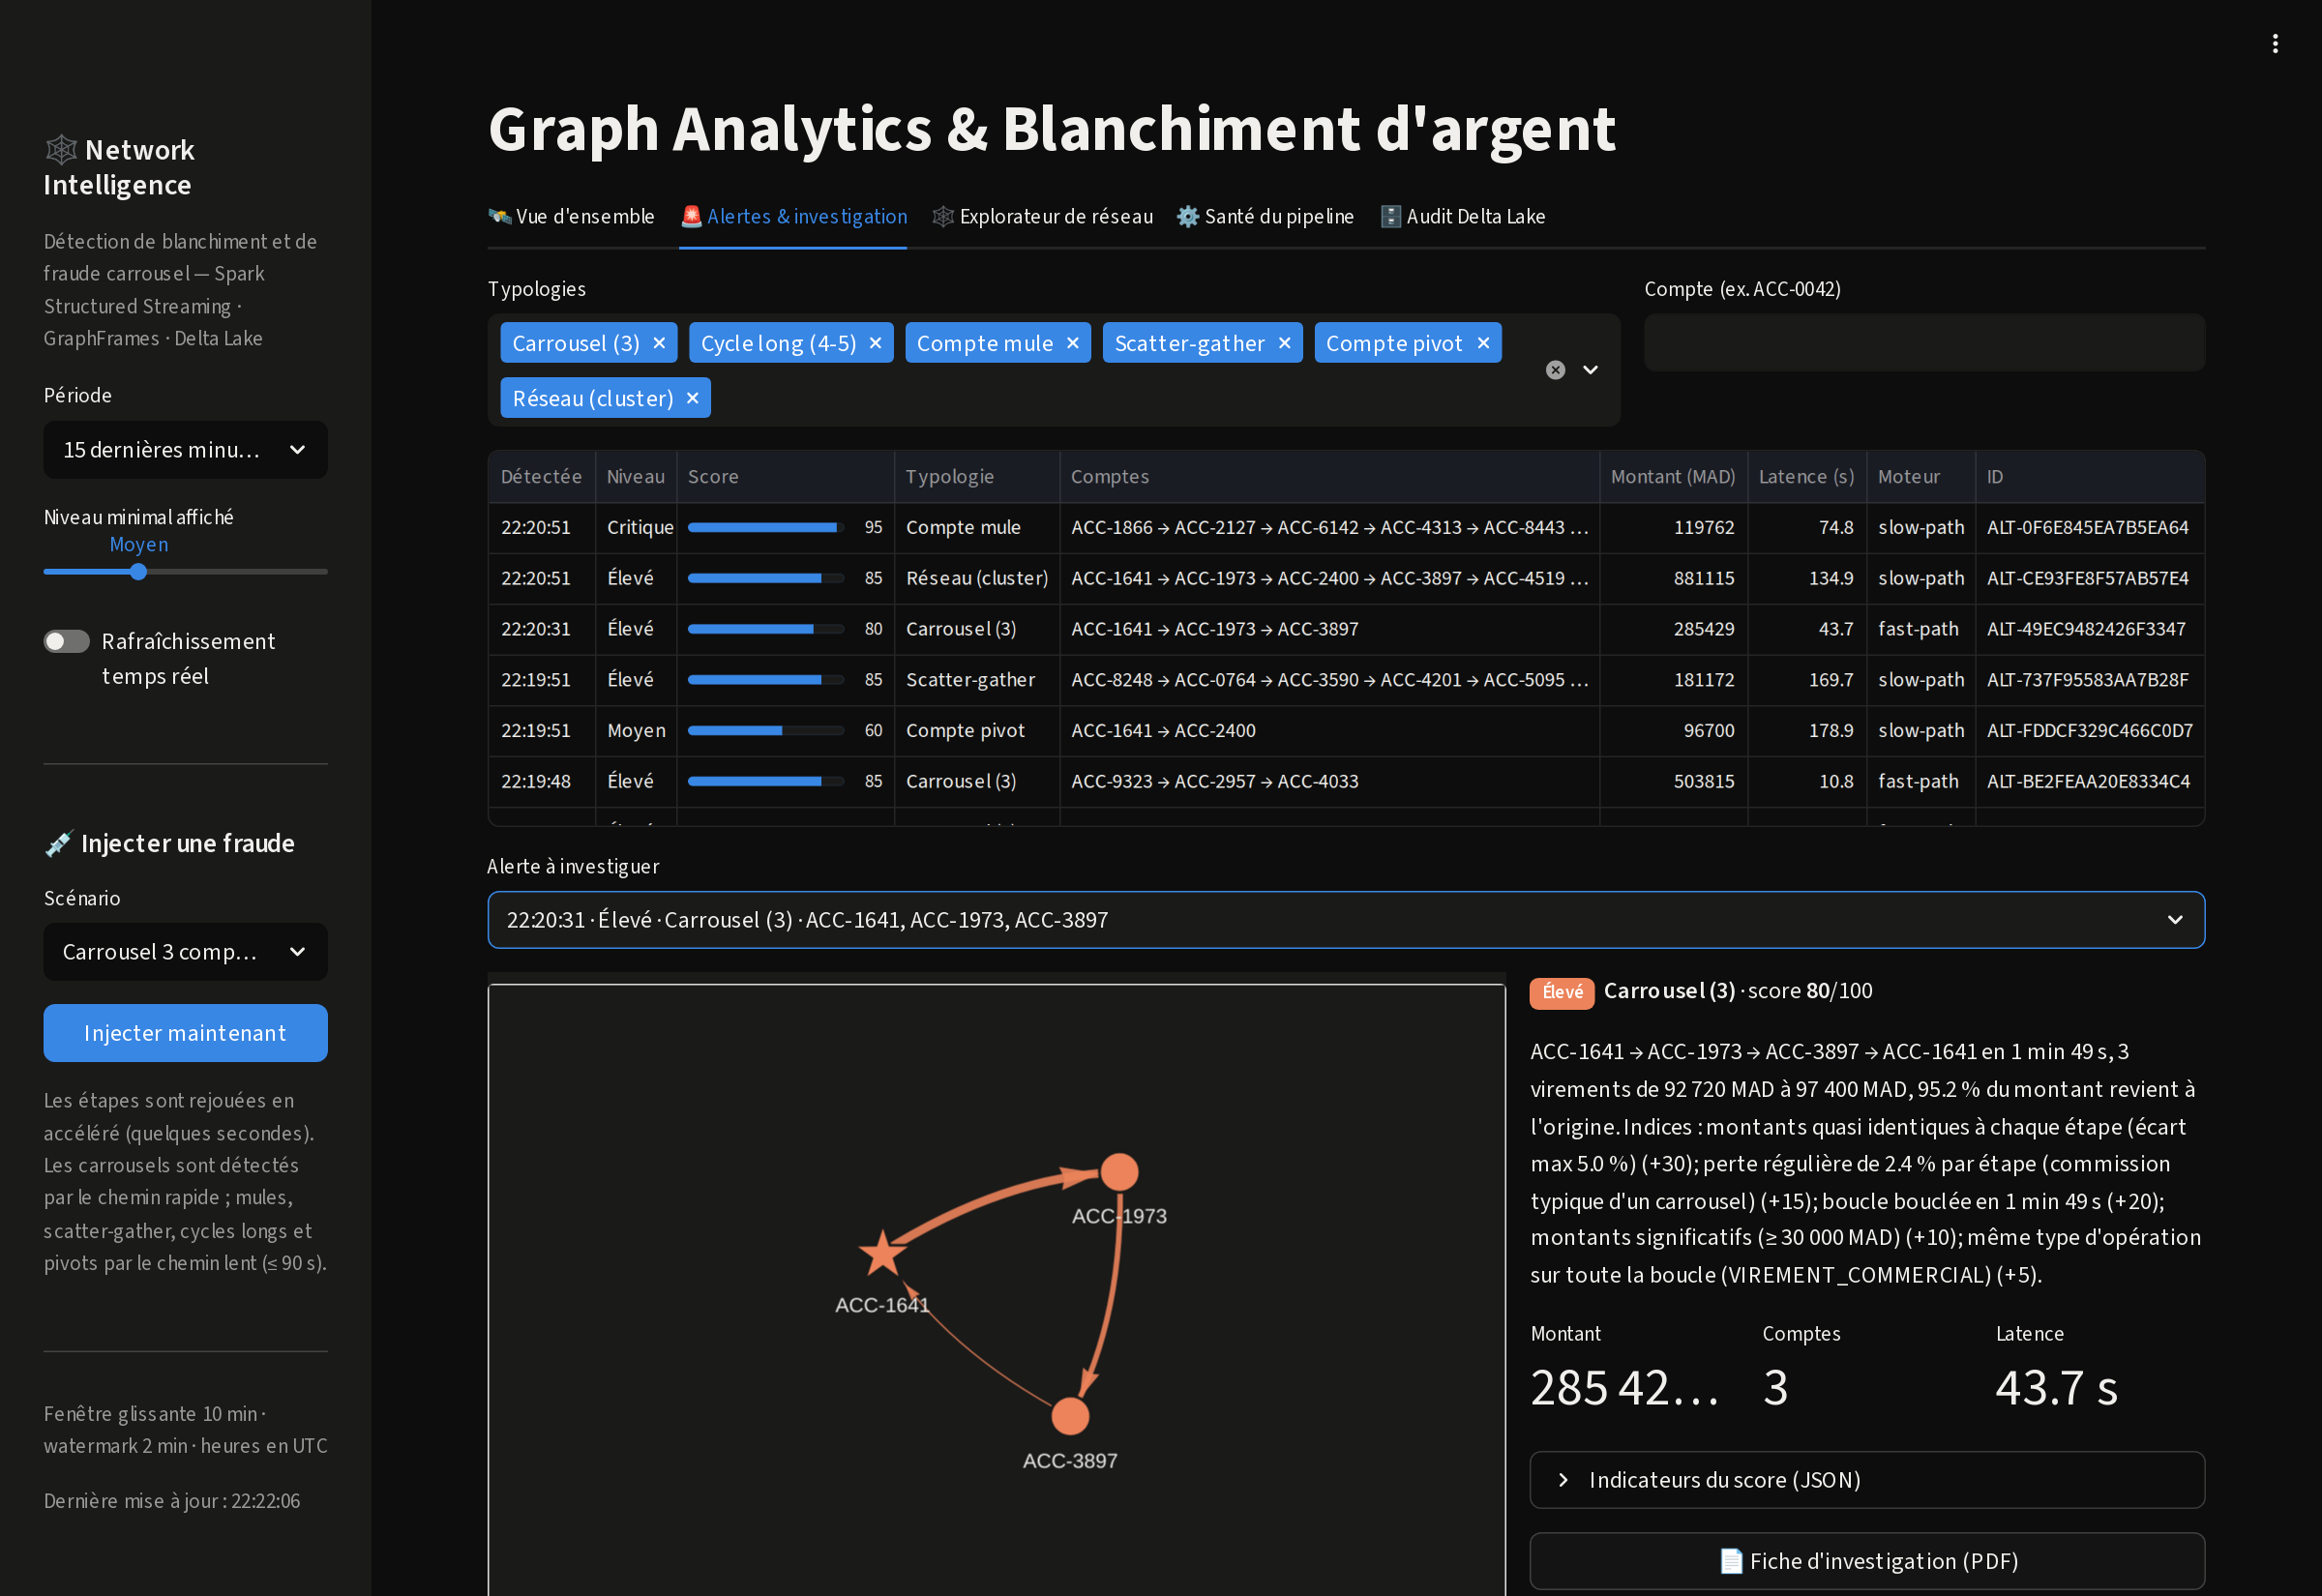
\includegraphics[width=0.495\linewidth]{figures/captures/dashboard_alertes.png}\hfill
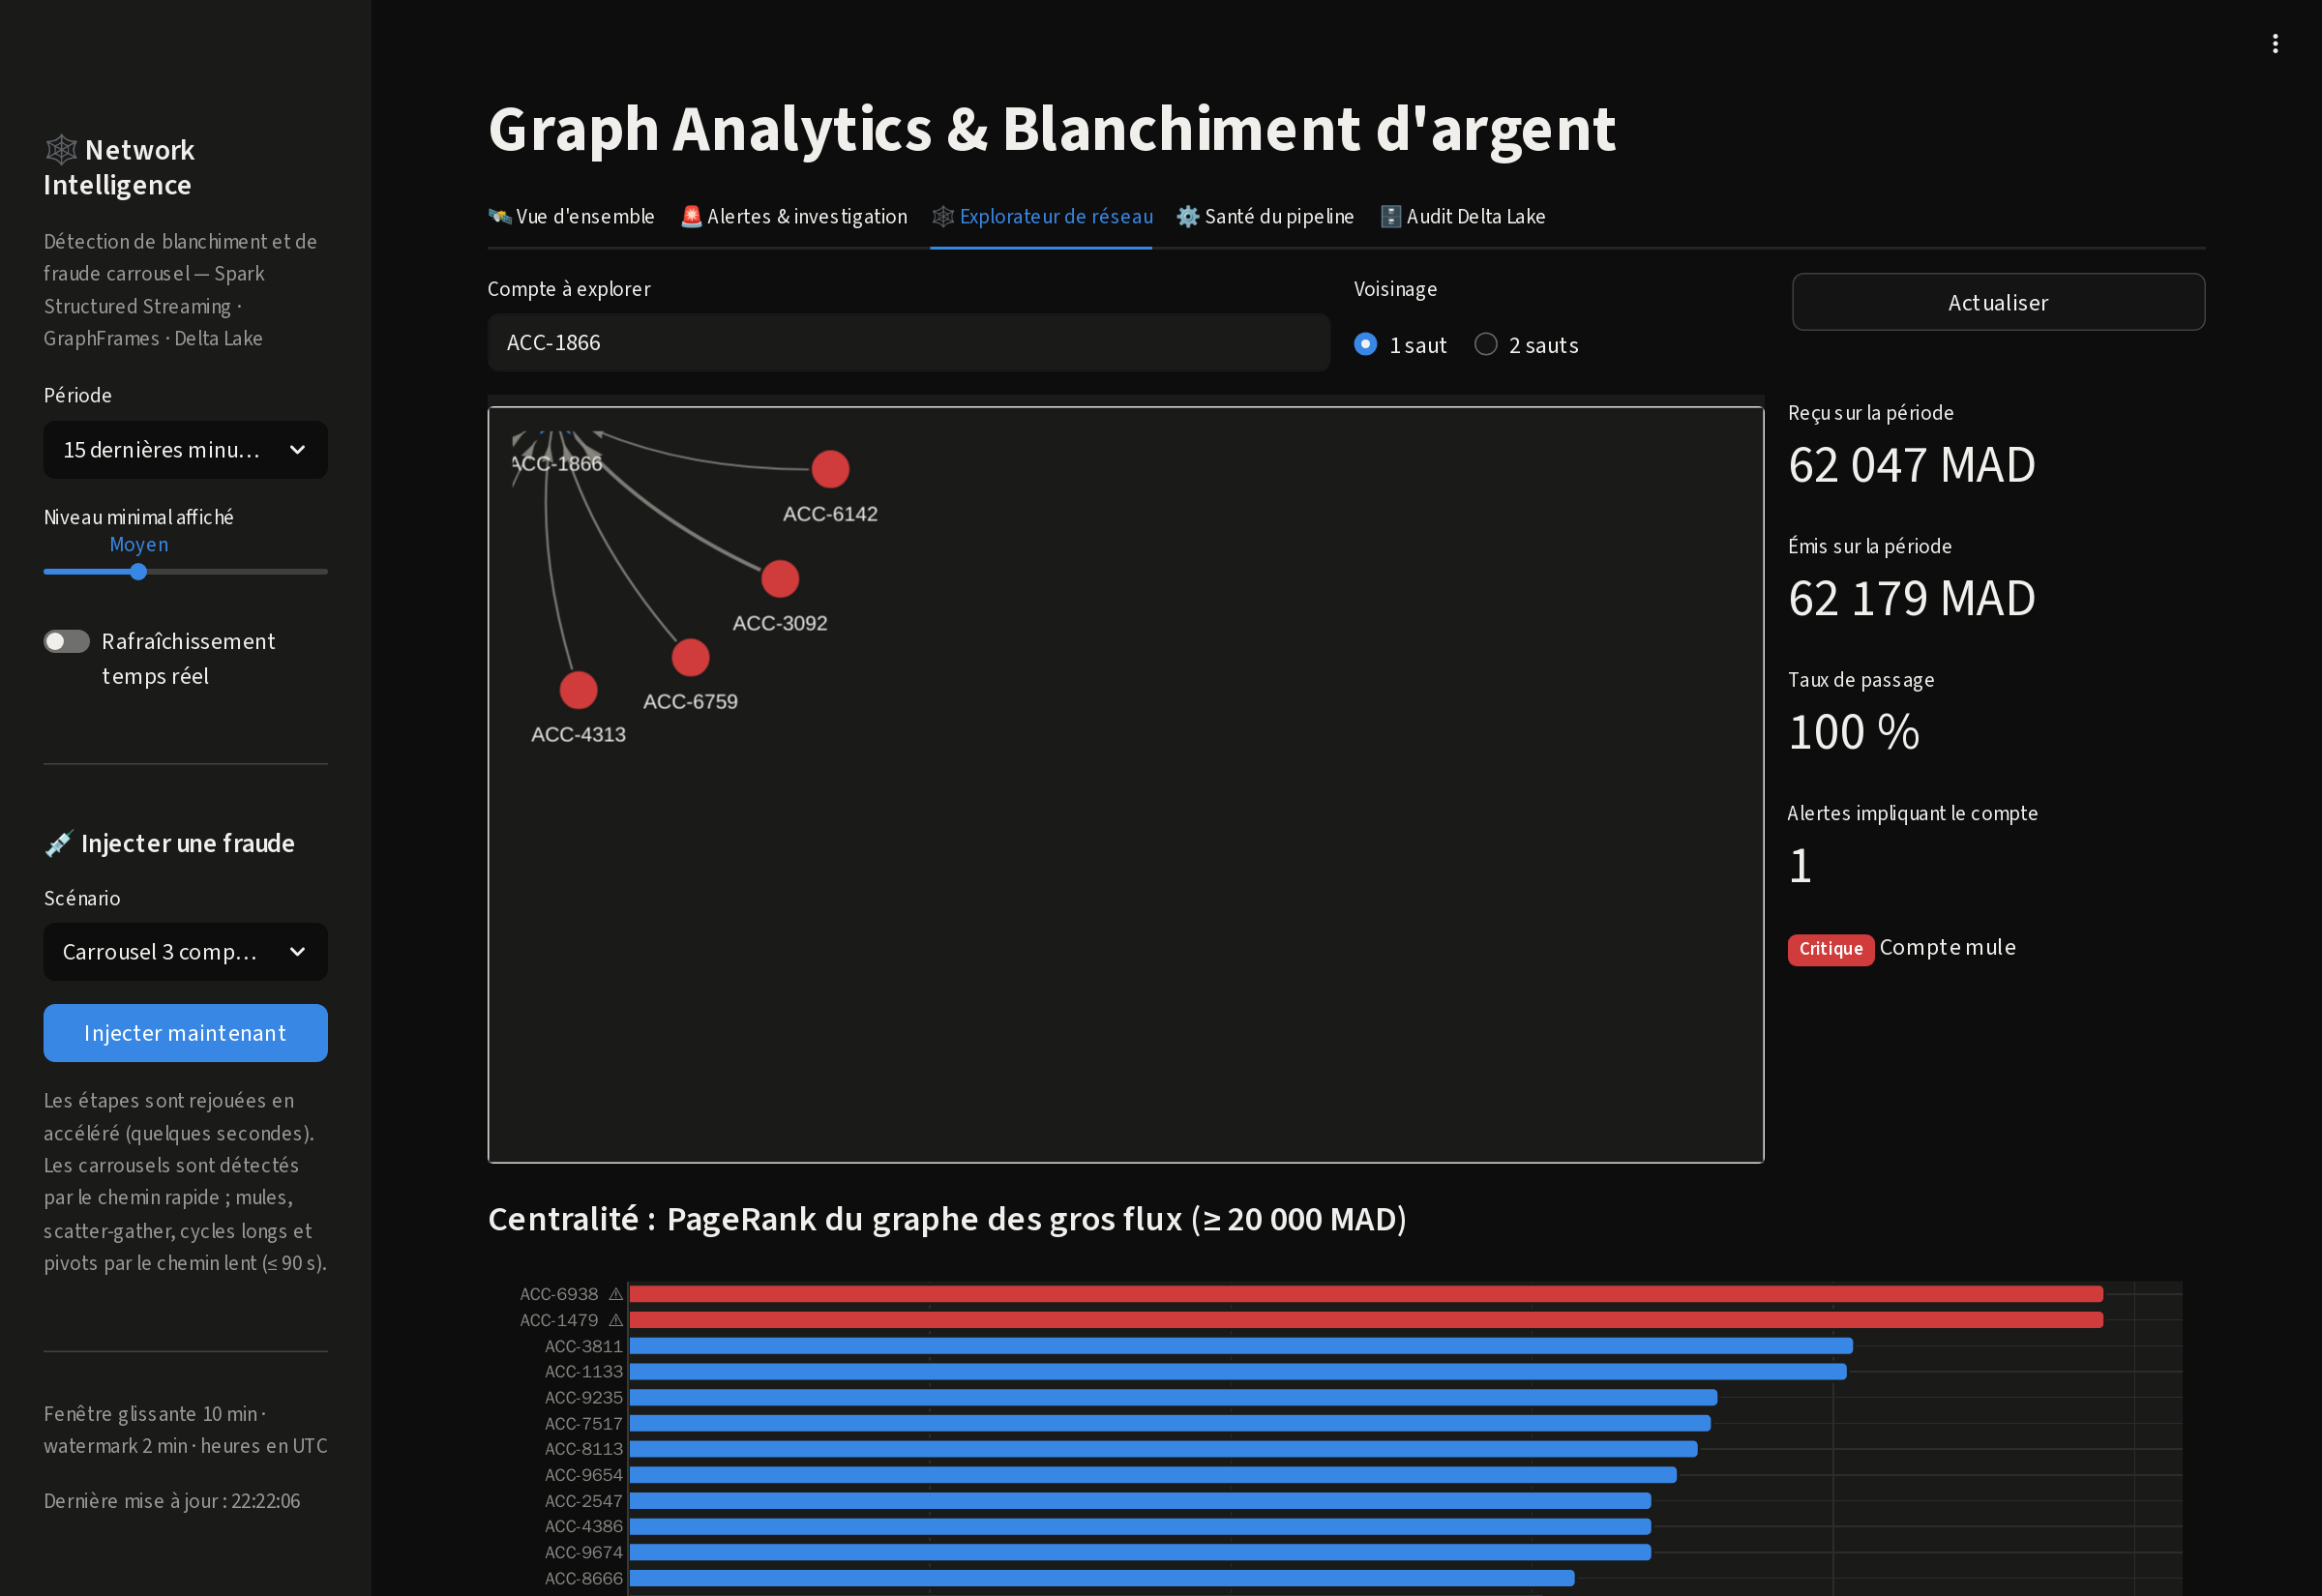
\includegraphics[width=0.495\linewidth]{figures/captures/dashboard_reseau.png}
\caption[Investigation d'une alerte et exploration du réseau]{À gauche, investigation d'une alerte :
sous-graphe interactif, score détaillé et fiche PDF téléchargeable. À droite, voisinage d'un compte
et classement PageRank du graphe des gros flux.}
\label{fig:dash2}
\end{figure}

\begin{figure}[htp]
\centering
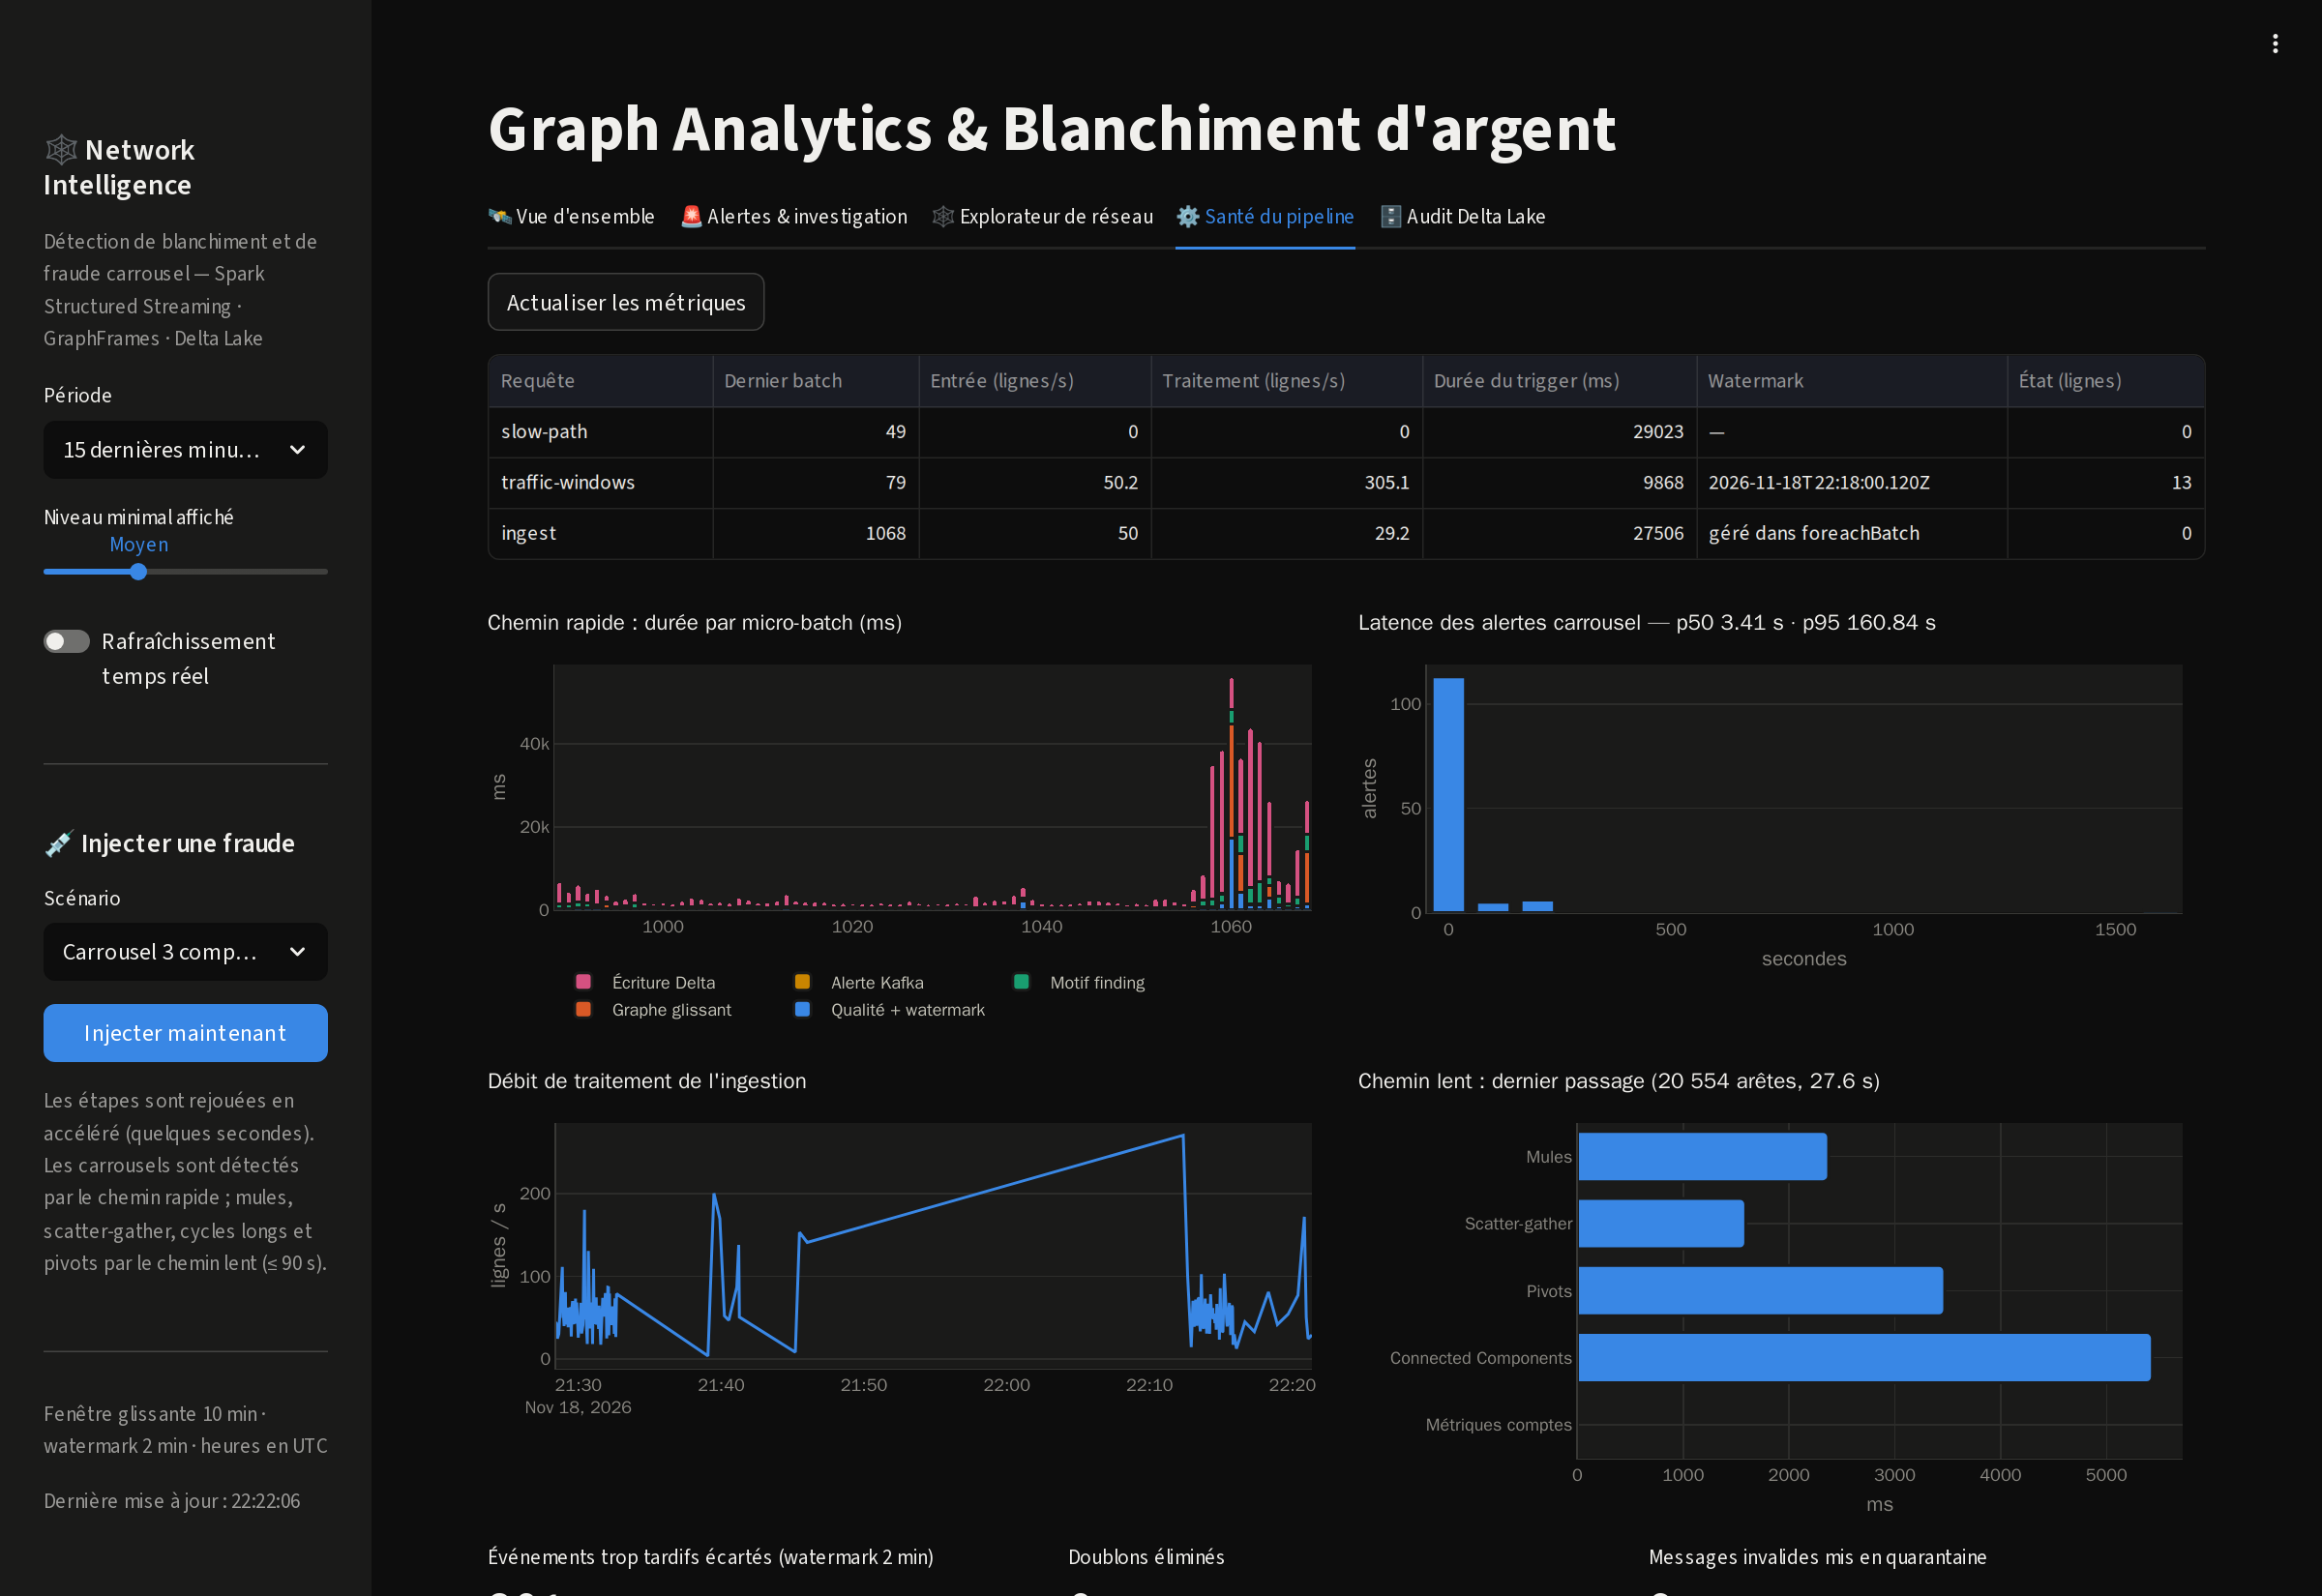
\includegraphics[width=0.495\linewidth]{figures/captures/dashboard_sante.png}\hfill
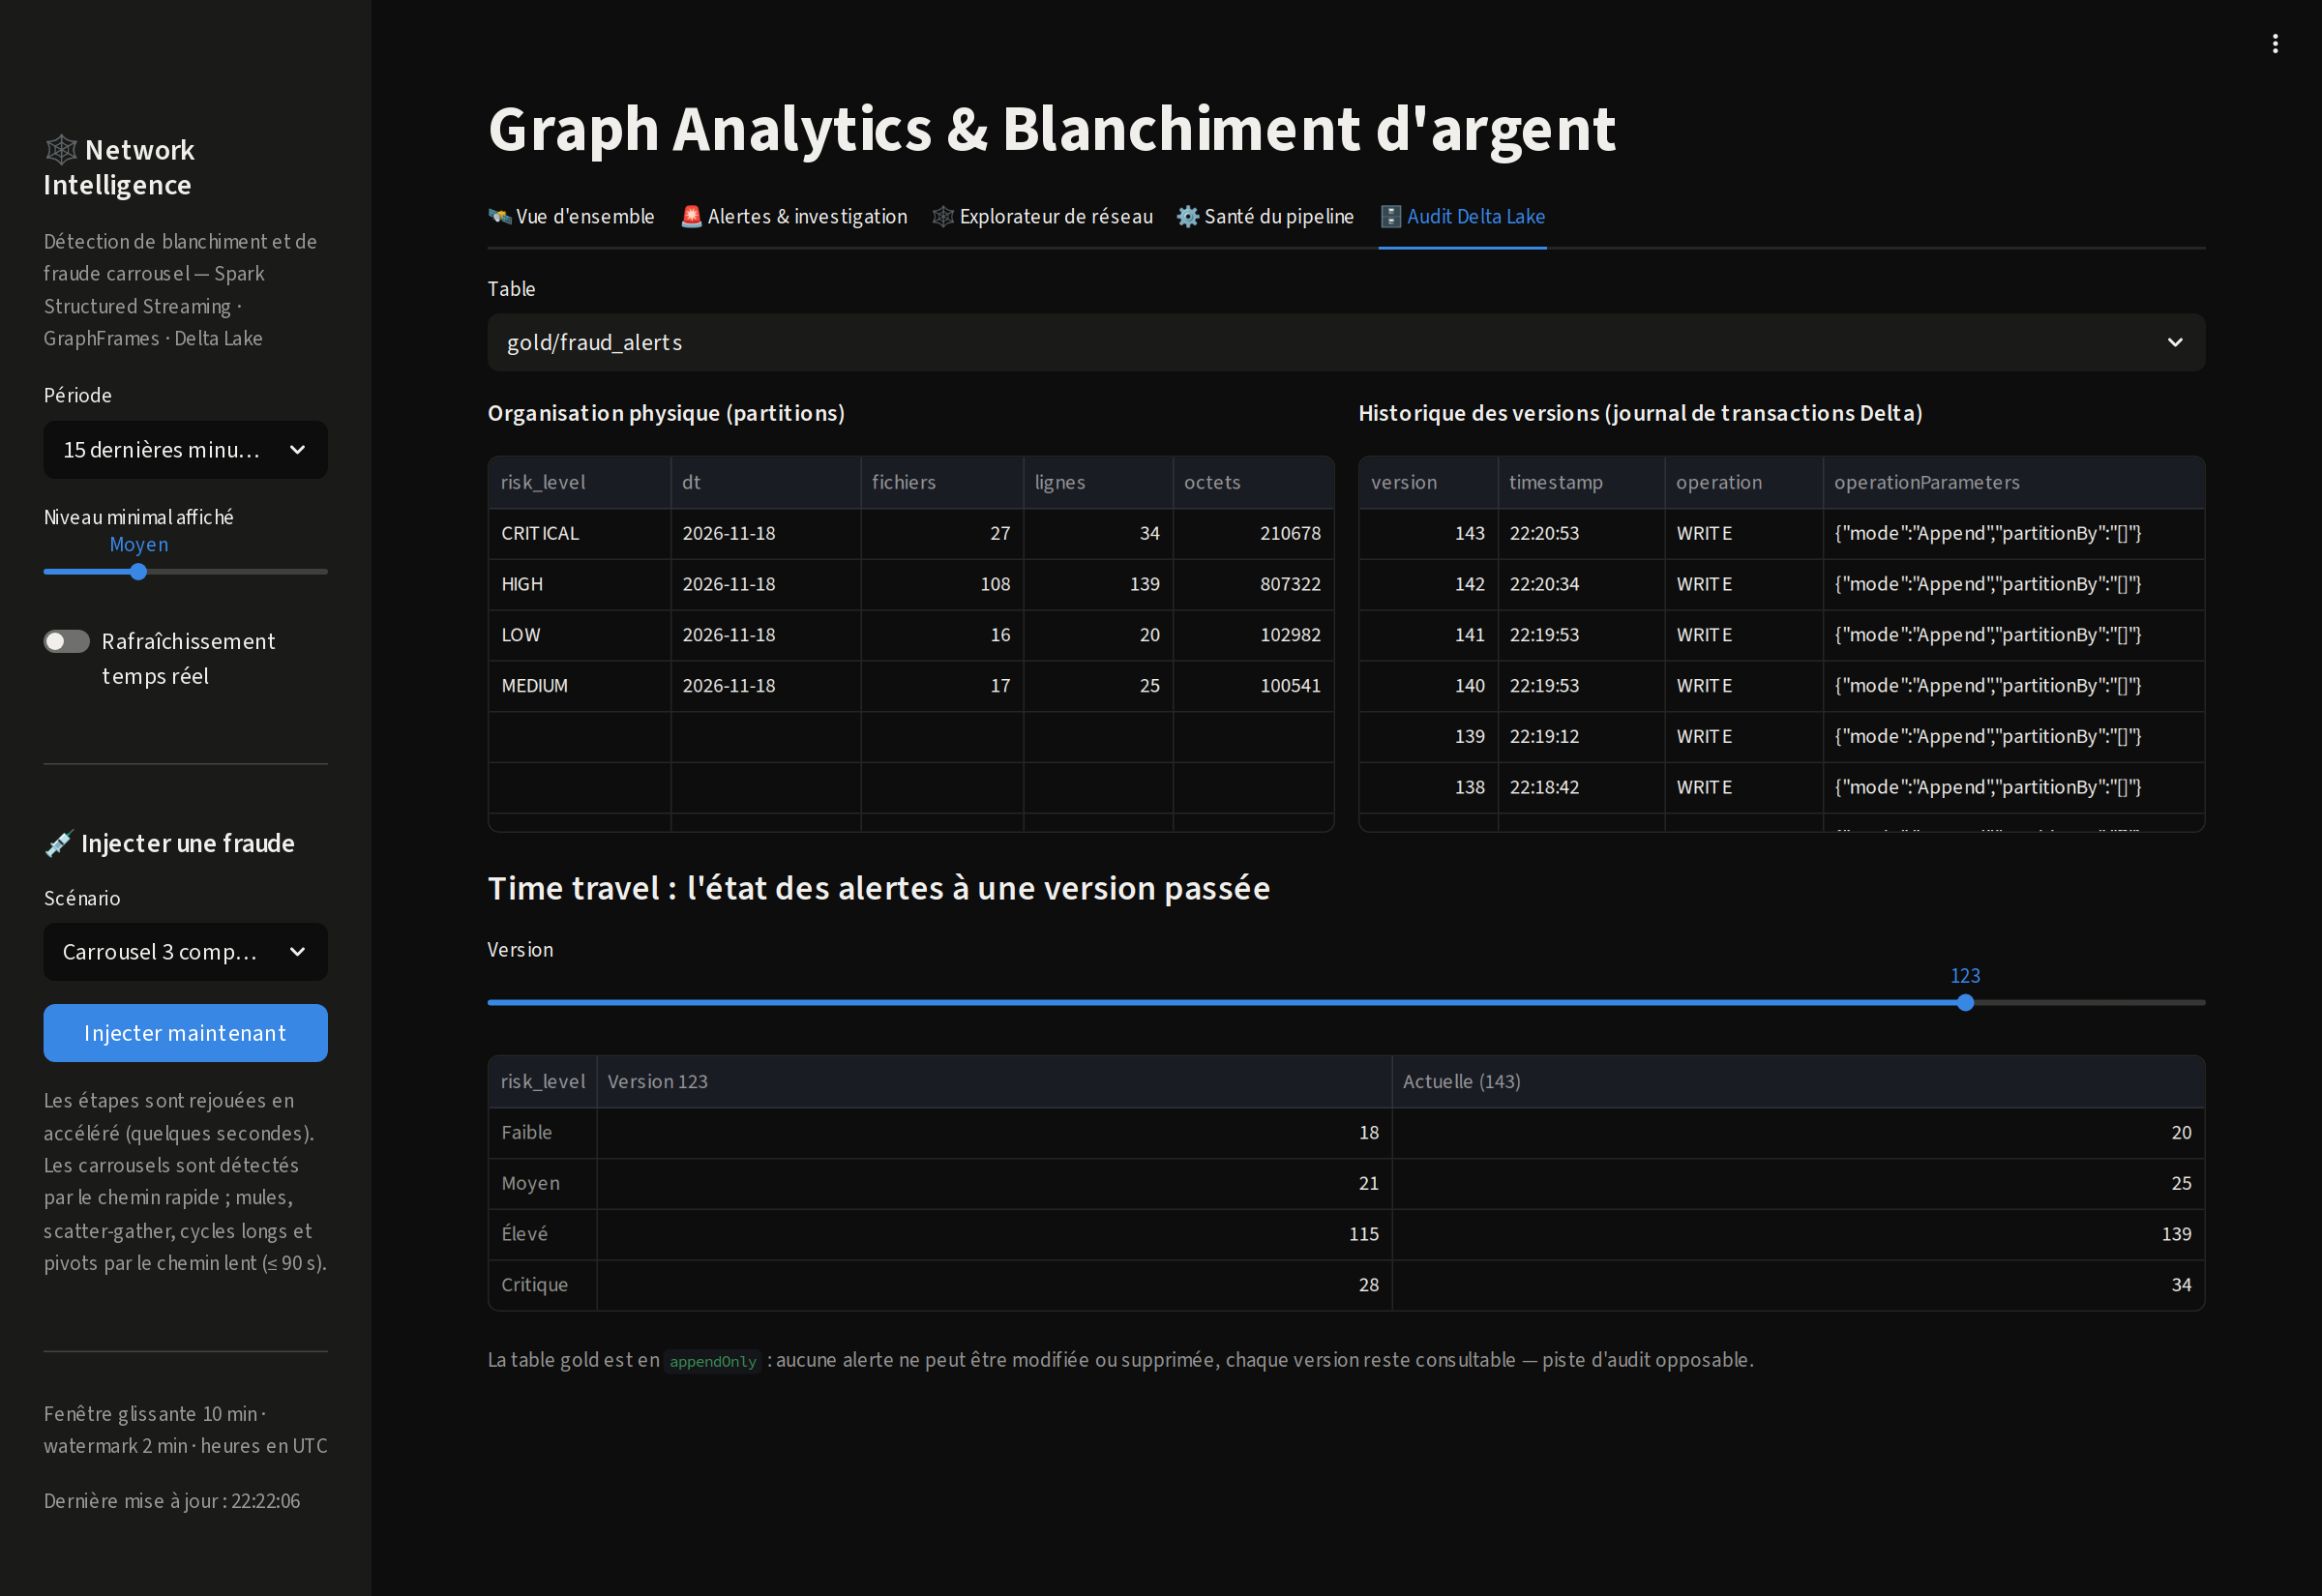
\includegraphics[width=0.495\linewidth]{figures/captures/dashboard_audit.png}
\caption[Santé du pipeline et audit Delta Lake]{À gauche, santé du pipeline : état des trois requêtes,
durée des micro-batchs décomposée par étape, latence des alertes. À droite, audit du lakehouse :
partitions, journal des versions et \emph{time travel} (état de la table des alertes à une version
passée).}
\label{fig:dash3}
\end{figure}

\section{La fiche d'investigation}
Pour chaque alerte, le tableau de bord produit une fiche PDF d'une page
(figure~\ref{fig:fiche}) : c'est le document qu'un analyste joindrait à une
déclaration de soupçon. Elle reprend l'explication en français, la liste
des comptes avec leur rôle et les virements du schéma, horodatés, et laisse
une place pour la décision de l'analyste.

\begin{figure}[htp]
\centering
\begin{minipage}[c]{0.46\linewidth}\centering
\fbox{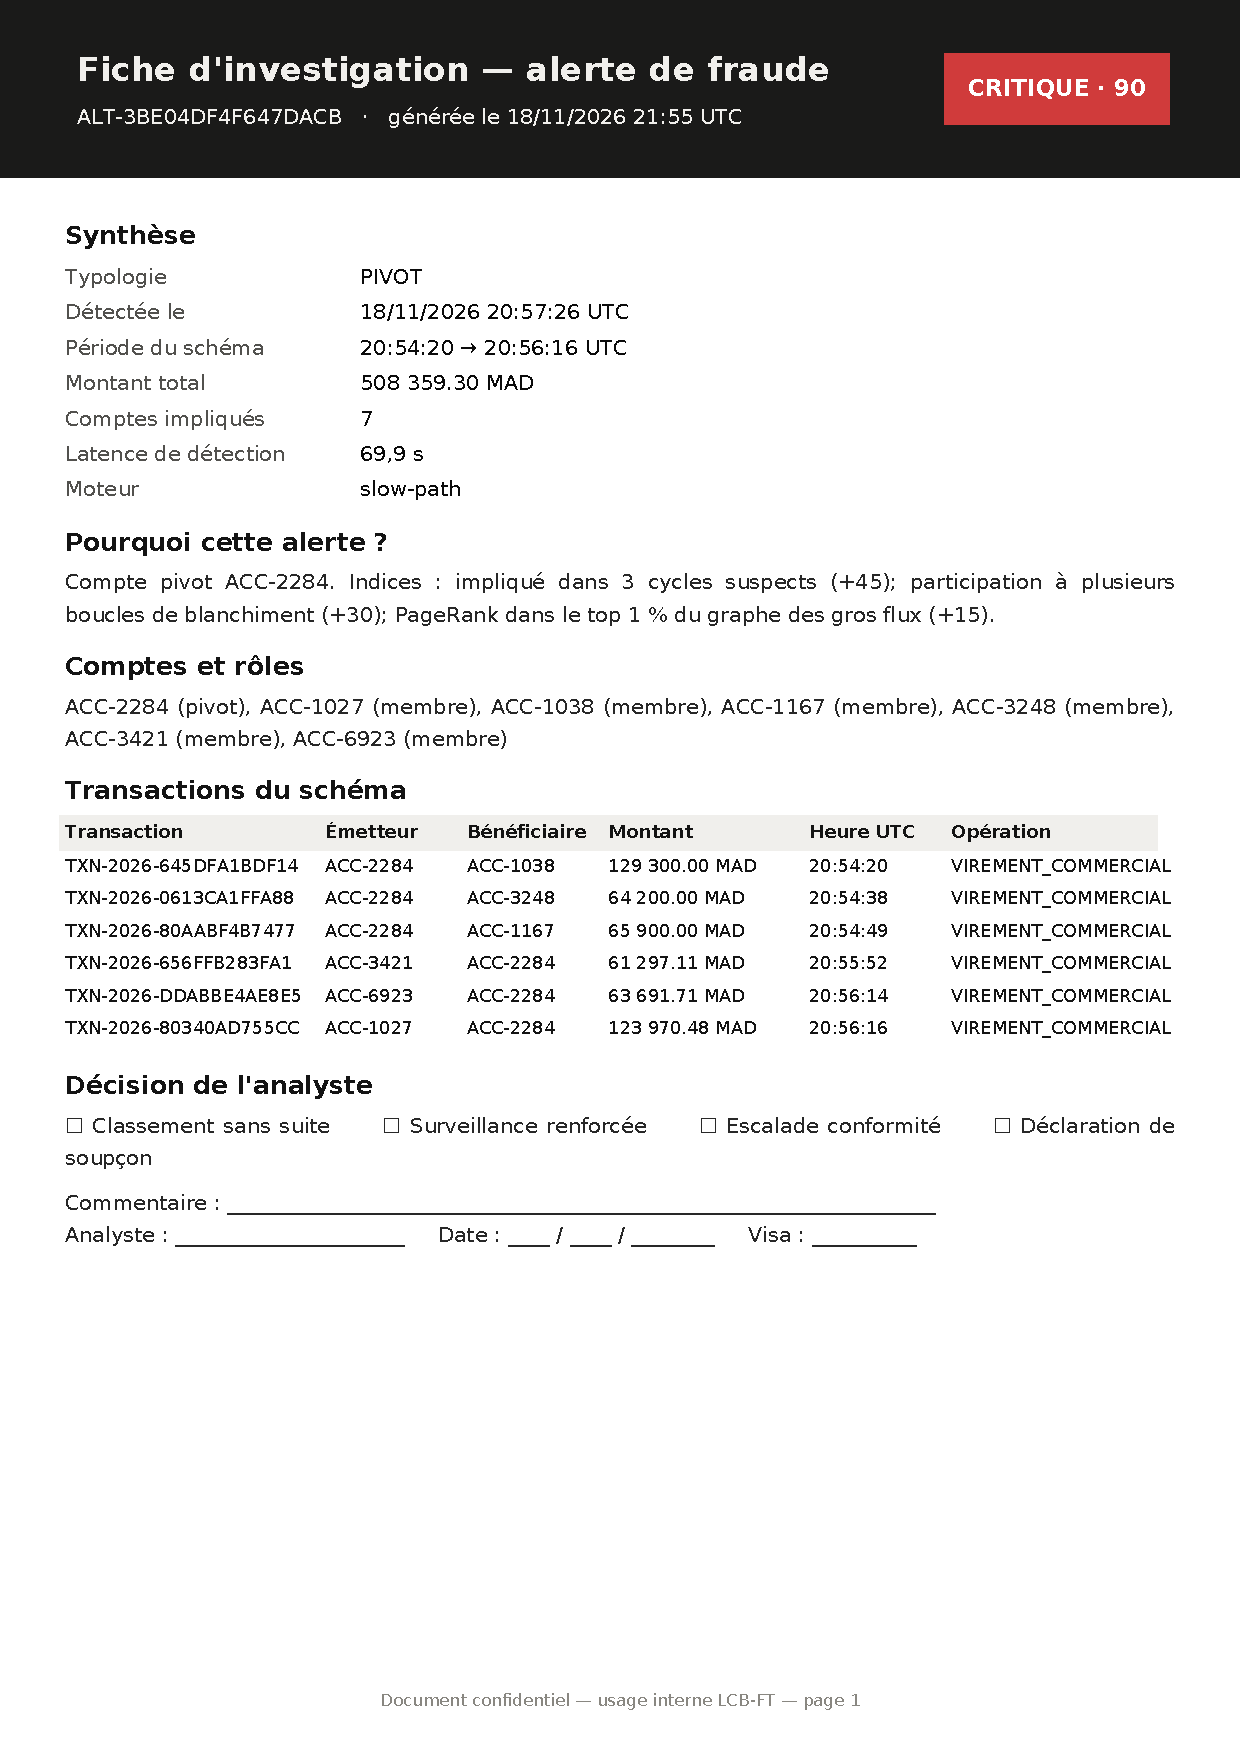
\includegraphics[width=0.92\linewidth]{figures/fiche_investigation.pdf}}
\end{minipage}\hfill
\begin{minipage}[c]{0.5\linewidth}
\begin{tikzpicture}[
  r/.style={font=\sffamily\scriptsize, text width=6.6cm, align=left, anchor=west},
  n/.style={circle, fill=bleuprojet, text=white, font=\sffamily\tiny\bfseries, minimum size=4mm, inner sep=0pt}]
  \foreach \i/\t [count=\k] in {
    1/{\textbf{En-tête} : identifiant de l'alerte, niveau et score},
    2/{\textbf{Synthèse} : typologie, période du schéma, montant, nombre de comptes, latence, moteur},
    3/{\textbf{Pourquoi cette alerte ?} L'explication en français, règle par règle},
    4/{\textbf{Comptes et rôles} dans le schéma (pivot, origine, mule, membre\ldots)},
    5/{\textbf{Transactions du schéma} : identifiant, émetteur, bénéficiaire, montant, heure},
    6/{\textbf{Décision de l'analyste} : classement, surveillance, escalade ou déclaration de soupçon, visa}} {
    \node[n] at (0,-\k*0.85) {\i};
    \node[r] at (0.3,-\k*0.85) {\t};
  }
\end{tikzpicture}
\end{minipage}
\caption[La fiche d'investigation PDF]{La fiche d'investigation générée pour une alerte PIVOT réelle du
run : le compte ACC-2284 au centre de trois carrousels (\fichier{fraud/report\_pdf.py}).}
\label{fig:fiche}
\end{figure}
